\documentclass[12pt]{article}
\usepackage[utf8]{inputenc}
\usepackage{amsmath}

\title{ECE 3413 Lab 02\\*Polynomials and Transfer Functions}
\author{Leomar Dur\'an}
\date{$9^{\text{th}}$ February 2023}

\usepackage{mathrsfs}
\usepackage{xfrac}
\usepackage{siunitx}

\usepackage{titling}
\usepackage{standalone}
\usepackage{pdfpages}

\usepackage{lib/nonfloatenvirons}
\usepackage{booktabs}
\newcommand\ra[1]{\renewcommand\arraystretch{#1}}
\ra{1.25}
\usepackage{minted}

\usepackage{matlab}
% \newcommand*\matlabtitle\subsection
% \newcommand*\matlabheading\subsubsection
% \newcommand*\mlcell[1]{#1}
% \newenvironment{matlaboutput}{%
    % \minted{matlab}%
% }%
% {%
    % \endminted%
% }%
% \newenvironment{matlabtableoutput}{}{}%

\usepackage{mathtools}%
\DeclarePairedDelimiter\brao()%
\DeclarePairedDelimiter\brac[]%
\DeclarePairedDelimiter\braco[)%
\DeclarePairedDelimiter\Brac\{\}%
\DeclarePairedDelimiter\norm\lVert\rVert%
\DeclarePairedDelimiter\piecefn\{.
\DeclarePairedDelimiter\evalat.|

\newcommand*\dd{d}

% save original spacing between paragraphs
\newlength\oldparskip
\setlength\oldparskip\parskip
% save new space between paragraphs
\newlength\newparskip
\setlength\newparskip\baselineskip
% commands for set/reset
\newcommand*\setparskip{\setlength\parskip\newparskip}
\newcommand*\resetparskip{\setlength\parskip\oldparskip}
% apply new space
\setparskip
% no indent
\setlength\parindent{0pt}

\def\hr{{\par\noindent\rule{\textwidth}{0.4pt}}}

\begin{document}

\maketitle
\newpage

\section{Introduction}

The purpose of this experiment is to reinforce and build on the introduction to Matlab from Lab 01.

This lab reviews operations on polynomials and teaches how to work with transfer functions.

In this example,
along with converting between the sum and factored forms of polynomials,
we will also experiment with converting between various forms of the transfer function,
namely ratio of polynomials, zero/pole/gain form and the time-domain form.

We will also review the circuit mesh analysis from Principles of Electric Circuits.

\section{Procedure}

\subsection{Parts 1.1, 1.2 -- Roots and polynomial forms}

We revisit the use of the representation of polynomials using row vectors of coefficients from highest to lowest order, 
as well as the use of \mintinline{matlab}{poly} to convert roots to the polynomials with those roots and
\mintinline{matlab}{roots} to convert polynomials to their roots.

\subsection{Part 1.3 -- Ratio of polynomials and zero/pole/gain forms}

We revisit the \mintinline{matlab}{tf} function that creates a transfer function as a ratio of polynomials and formally introduce the \mintinline{matlab}{zpk} mentioned in Lab 01. This latter function creates a transfer function as a vector of zeroes, a vector of poles, and the gain.

\subsubsection{Conversion between transfer function forms}

In addition to creating transfer functions from vectors, 
\mintinline{matlab}{tf} and \mintinline{matlab}{zpk} can be used to convert back and forth between the different forms of transfer functions.

\subsection{Part 1.4 -- Partial fraction expansion}

\subsubsection{Purpose}

The reason for partial fraction decomposition is preparation for the inverse Laplace transform.
The inverse Laplace transform expects the function to be transformed to have a form such as the ones in the $F\brao*s$ column of Table \ref{tab:laplace}.
Partial fraction decomposition helps us meet that goal.

\begin{table}[h!]
    \centering
    \caption{Laplace transforms.}
    \[
        \begin{array}{@{}ll@{}}
            \toprule
                f\brao*t & F\brao*s
            \\*
            \midrule
                t^n u\brao*t
                    & \dfrac{n!}{s^{n+1}}
            \\*[0.75em]
                e^{-at}u\brao*t
                    & \dfrac{1}{s+a}
            \\*[0.75em]
                \cos\brao*{\omega t}u\brao*t
                    & \dfrac{s}{s^2 + \omega^2}
            \\*[0.75em]
                \sin\brao*{\omega t}u\brao*t
                    & \dfrac\omega{s^2 + \omega^2}
            \\*
            \bottomrule
        \end{array}
    \]
    \label{tab:laplace}
\end{table}

For example, let's say we have
\begin{equation}
    G_5\brao*s = \frac{5\brao{s + 2}}{s\brao{s^2 + 6s + 34}}.
\end{equation}

It is necessary first to perform partial fraction decomposition and rewrite it in a form
\begin{equation}
    G_5\brao*s = \frac{A}s + \frac{Bs + C}{s^2 + 6s + 34},
\end{equation}
where the denominators are each as factored out as they can be.
This produces
\begin{equation}
    G_5\brao*s = \frac{\sfrac{10}{34}}s + \frac{\brao{\sfrac{-10}{34}}s + \sfrac{110}{34}}{s^2 + 6s + 34}.
\end{equation}

\paragraph{What next?}

The denominator of the second fraction $s^2 + 6s + 34$ should be in the form $\hat{s}^2 + \omega^2$ in Table \ref{tab:laplace}.
(Note that this is not the same $s$ as in $G_5\brao*s$, so we will refer to it as $\hat{s}$.) In other words, $s^2 + 6s + 34$ must be a sum of two squares.

To find the first square $\hat{s}^2$, we need to complete the first square.
``Completing the square'' refers to the rule $\brao{a - b}^2 = a^2 - 2ab + b^2$.
We can find $b^2$ if we know $a^2$ and $2ab$.
Well $a^2 = s^2$ and $2ab = 6s$.
Thus $a = s$, and $-2ab = 2s\brao*b = 6s$.
So $b = -\sfrac62 = -3$.
This makes $b^2 = \brao{-3}^2 = 9$.

We now know that $s^2 + 6s + 34 = \brao{s^2 + 6s + 9} + \omega^2 = s^2 + 6s + \brao{9 + \omega^2}$.
Thus $9 + \omega^2 = 34$.
We have $\omega = \sqrt{25} = 5$.

So $s^2 + 6s + 34 = \brao{s^2 + 6s + 9} + 5^2$.
Now we can factor $a^2 - 2ab + b^2$ to $\brao{a - b}^2$. So $s^2 + 6s + 34 = \brao{s + 3}^2 + 5^2$, and more specifically, we have
\begin{equation}
    \piecefn*{
        \begin{matrix}
            \hat{s} = s + 3,
        \\*
            \omega = 5.
        \\*
        \end{matrix}
    }
\end{equation}

Our transfer function now has the form
\begin{equation}
    G_5\brao*s = \frac{\sfrac{10}{34}}s + \frac{\brao{\sfrac{-10}{34}}s + \sfrac{110}{34}}{\brao{s + 3}^2 + 5^2}.
\end{equation}

The last step is splitting the second function into $\sfrac{\hat{s}}{\brao*{\hat{s}^2 + \omega^2}}$ and $\sfrac\omega{\brao*{\hat{s}^2 + \omega^2}}$ forms.
Since the denominator is already in the correct form, we need to split the numerator.
\begin{equation}
    \brao{\sfrac{-10}{34}}s + \sfrac{110}{34} = D\hat{s} + E\omega = D\brao{s + 3} + E\brao5.
\end{equation}

Well, $D = \sfrac{-10}{34}$ by inspection of the $s^1$ coefficients, so that leaves
\begin{equation}
    \frac{110}{34} = -\frac{10}{34}\brao3 + E\brao5
\end{equation}
Thus $E = \sfrac{28}{34}.$

Finally, we have 
\begin{equation}
    G_5\brao*s = \frac{\sfrac{10}{34}}s + \frac{\brao{\sfrac{-10}{34}}\brao*{s + 3}}{\brao{s + 3}^2 + 5^2}  + \frac{\brao{\sfrac{28}{34}}3}{\brao{s + 3}^2 + 5^2}
\end{equation}
which is ready for inverse Laplace transformation.
The coefficients may be extracted from the numerators giving
\begin{equation}
    G_5\brao*s = \brao*{\frac{10}{34}}\frac1s - \brao*{\frac{10}{34}}\frac{\brao*{s + 3}}{\brao{s + 3}^2 + 5^2}  + \brao*{\frac{28}{34}}\frac{3}{\brao{s + 3}^2 + 5^2}.
\end{equation}


\subsubsection{Storing transfer functions}

To store transfer functions,
I chose to store them each as a numerator and denominator, storing 2 factors, each potentially as trinomials.
The factors are then multiplied.

I could have used the ZPK model, but this would have required a separate vector for the gains.

Now when a polynomial with $S + 1$ terms is multiplied with a polynomial with $T + 1$ terms, the resulting vector will be of length $S + T + 1$,

Now if we multiply together $2$ polynomials both with $S + 1$ terms,
we will have a product polynomial with $2S + 1$ terms,
and $3$ polynomials this is the same as a polynomial with $2S + 1$ terms and a polynomial of $S + 1$ terms, which
will give $\brao*{2S} + \brao*{S} + 1 = 3S + 1$ terms.
Thus, multiplying $P + 1$ polynomials with $S + 1$ terms will produce a polynomial with $\brao*{P + 1}S + 1$ terms.

Let $Q := P + 1$ and $T = S + 1$, then multiplying $Q$ polynomials with $T$ terms each will produce a polynomial of $Q\brao*{T - 1} + 1$ terms. Thus, we can store the numerator and denominator of each polynomial in $2\brao*{3 - 1} + 1 = 5$ terms.

\subsubsection{Partial fraction decomposition in Matlab}

Matlab provides the \mintinline{matlab}{residue} function which accepts a fraction as a vector of coefficients for numerator and another for denominator,
returning a vector of its partial fraction numerators, the corresponding poles of the fractions and the direct function,
which is the quotient polynomial resulting by dividing the numerator of the original fraction by its denominator.
In the case of a proper rational expression there is no direct function.
Now Simulink does not allow you to realize an improper rational expression as a transfer function as seen in Fig \ref{fig:error:improper transfer function}.
So I believe this means that it would not be a legal transfer function.

\begin{figure}[h!]
    \centering
    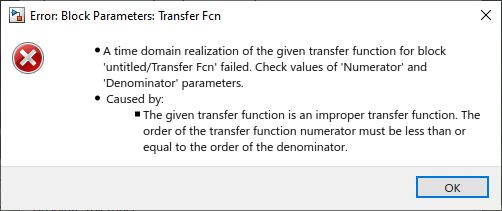
\includegraphics[width=0.8\linewidth]{improper_transfer_function.png}
    \caption{Error from attempting to realize an improper rational expression as a transfer function.}
    \label{fig:error:improper transfer function}
\end{figure}

The \mintinline{matlab}{residue} function has its disadvantages.
First, the function does not differentiate between repeated roots, at least not within its documentation.
The order of the roots is not documented, but from the results, it seems to be
\begin{enumerate}
    \item first by real part from lowest to highest;
    \item then by imaginary part from highest to lowest;
    \item then in the case of repeat roots, by order of the polynomial giving that root (\textit{i.e.}, $s+1$ before $\brao{s+1}^2$).
\end{enumerate}

Since this is not documented, it may be subject to change, but for now it works.
I used this knowledge to convert the partial fraction decompositions from vectors to symbolic objects for display in a Matlab Live Script.

The second disadvantage is that algorithm factors out the denominator down to the monomial, even when this will result in a complex root.
This is by design, and it will likely be more useful in this course,
but the expected behavior is not to factor out polynomials that will have complex roots.
That is, the coefficients and constant term of a polynomial are usually expected to be real numbers (with $1$ being the coefficient of the highest order term).
Since this is the default behavior in Matlab, I have left it as is.

\subsection{Part 2 -- Laplace transforms and inverse Laplace transforms}

The Laplace transform is used to convert a fraction from time-domain to frequency domain.

Both the Laplace transform function \mintinline{matlab}{laplace}
and the inverse Laplace transform function \mintinline{matlab}{ilaplace} in Matlab are
very straightforward and give you almost what you would expect.

The only difference is that Matlab does not represent time-domain form by having the Heaviside step function $u\brao*t$ as a factor.

Additionally, I chose to add a section to part 2.1 that performs the inverse Laplace transform on transfer functions in zero/pole/gain form for consistency with the other ways that transfer functions are handled.

\subsection{Part 3 -- Review of solving circuit loops}

We are given the circuit in Fig. \ref{fig:circuit}.

\begin{figure}[h!]
    \centering
    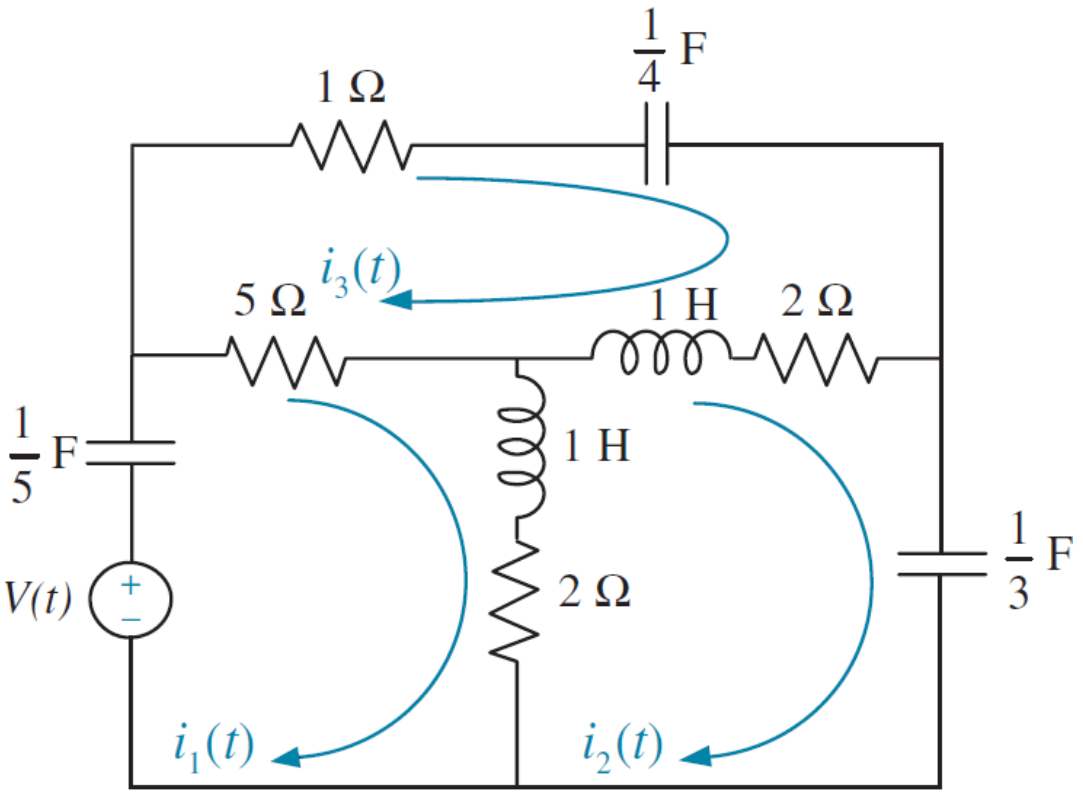
\includegraphics[width=0.5\linewidth]{part03_circuit.png}
    \caption{We must find the current loops in this circuit.}
    \label{fig:circuit}
\end{figure}

We start by labeling the polarities and components as in Fig. \ref{fig:circuit labeled}.
As with the directions in finding the reaction forces in a mechanical problem, these polarities are guesses and may be updated later.
As a convention, we label the first terminal met by the current as positive and the second terminal as negative.
There is no convention for labeling the components. It is just a way to differentiate them.

\begin{figure}[h!]
    \centering
    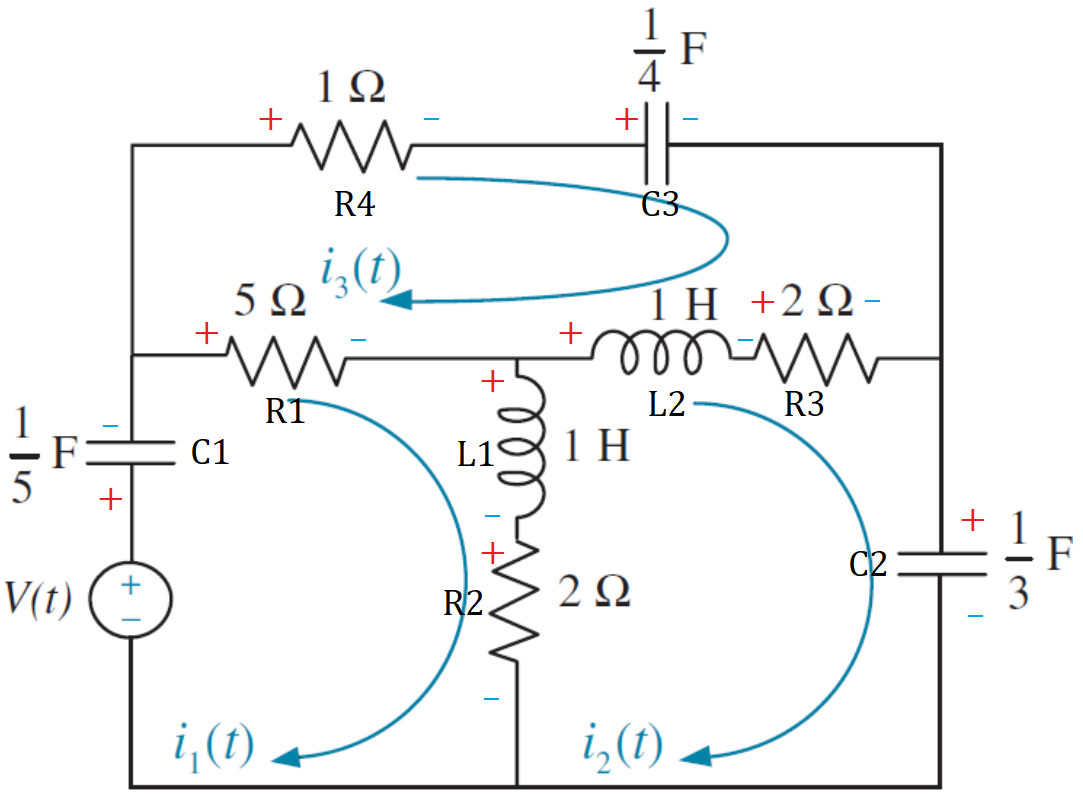
\includegraphics[width=0.5\linewidth]{part03_circuit-labeled.png}
    \caption{The circuit with polarities and components labeled.}
    \label{fig:circuit labeled}
\end{figure}

Let's start with loop $i_1\brao*t$.
We apply Kirchhoff's voltage law, which states that the sum of all currents around a loop are zero. 
We use the first terminal's polarity with the current as the sign of the voltage, starting with the voltage source $V\brao*t$. (That is, voltage rises are noted as negative, and voltage drops are noted as positive.)

\begin{equation}
    \begin{array}{@{}ll@{}}
        \operatorname{KVL}: & 0 = \sum V = -V\brao*t + V_{C1} + V_{R1} + V_{L1} + V_{R2}
    \end{array}
\end{equation}

Next we rewrite these voltages in terms of currents, except for the voltage source, according to \ref{eq:voltage equations}.
Remember that the inductor $L_1$ and resistor $R_2$ on the right-hand side of the loop are also in loop $i_2\brao*t$, and resistor $R_1$ at the top of the loop is also in loop $i_3\brao*t$.
Notice that when two voltages move in the same direction through the component, we add them. When they clash, we subtract the other current from the one with which we are working.

\begin{equation}\label{eq:voltage equations}
    \piecefn*{
        \begin{matrix}        
            V_R = IR,
        \\*
            v_L = L D_t i,
        \\*[0.75em]
            v_C = \dfrac1C \displaystyle\int_0^t i\brao\tau d\tau.
        \\*
        \end{matrix}
    }
\end{equation}

\begin{equation}
    0 = -V\brao*t + \dfrac1{C_1} \displaystyle\int_0^t i_1\brao\tau d\tau + R_1 \brao{i_1 - i_3}\brao*t + \brao*{L_1 D_t +  R_2}\brao{i_1 - i_2}\brao*t.
\end{equation}

Finally, we may take the Laplace transforms, which give us

\begin{equation}
    0 = -\mathscr{L}\brac{V\brao*t}\brao*s + \frac1{sC_1} I_1\brao*s + R_1 \brao{I_1 - I_3}\brao*s + \brao*{sL_1 + R_2}\brao{I_1 - I_2}\brao*s.
\end{equation}

We group together like current terms

\begin{equation}
    \mathscr{L}\brac{V\brao*t}\brao*s = \brao*{\frac1{sC_1} + R_1 + sL_1 + R_2} I_1\brao*s + \brao*{-sL_1 - R_2} I_2\brao*s - R_1 I_3\brao*s.
\end{equation}

We do the same for loop $i_2\brao*t$, first finding the sum of the voltage across components

\begin{equation}
    0 = \frac1{sC_2} I_2\brao*s +\brao*{R_2 + sL_1}\brao{-I_2 + I_1}\brao*s + \brao*{sL_2 + R_3}\brao*{I_2 - I_3}\brao*s,
\end{equation}

then grouping like current terms

\begin{equation}
    0 = \brao*{R_2 + sL_1}I_1\brao*s + \brao*{\frac1{sC_2} - R_2 - sL_1 + sL_2 + R_3} I_2\brao*s + \brao*{-sL_2 - R_3}I_3\brao*s.
\end{equation}

We repeat for loop $i_3\brao*t$.

\begin{equation}
    0 = \brao*{R_4 + \frac1{sC_3}} I_3\brao*s + \brao*{R_3 + sL_2}\brao*{-I_3 + I_2}\brao*s + R_1\brao*{-I_3 + I_1}\brao*s,
\end{equation}
then
\begin{equation}
    0 = R_1 I_1\brao*s + \brao*{R_3 + sL_2}I_2\brao*s + \brao*{R_4 + \frac1{sC_3} - R_3 + sL_2 - R_1}I_3\brao*s.
\end{equation}

Thus we have the system of equations.

\begin{equation}
    \hskip-5em
    \begin{aligned}
        &\brac*{
            \begin{matrix}
                \brao*{\frac1{sC_1} + R_1 + sL_1 + R_2} & \brao*{-sL_1 - R_2} & R_1
            \\*
                \brao*{R_2 + sL_1} & \brao*{\frac1{sC_2} - R_2 - sL_1 + sL_2 + R_3} & \brao*{-sL_2 - R_3}
            \\*
                R_1 & \brao*{R_3 + sL_2} & \brao*{R_4 + \frac1{sC_3} - R_3 + sL_2 - R_1}
            \\*
            \end{matrix}
        }\brac*{
            \begin{matrix}
                I_1 \\* I_2 \\* I_3 \\*
            \end{matrix}        
        }%
        \brao*s
    \\*
        ={}&
        \brac*{
            \begin{matrix}
                \mathscr{L}\brac{V\brao*t}\brao*s \\* 0 \\* 0 \\*
            \end{matrix}
        }
    \end{aligned}
\end{equation}

We use Matlab to solve the system of equations in Appendix \ref{apx:solving circuit loops}.

\section{Results}

\hr
\resetparskip
% This LaTeX was auto-generated from MATLAB code.
% To make changes, update the MATLAB code and export to LaTeX again.

\documentclass{article}

\usepackage[utf8]{inputenc}
\usepackage[T1]{fontenc}
\usepackage{lmodern}
\usepackage{graphicx}
\usepackage{color}
\usepackage{hyperref}
\usepackage{amsmath}
\usepackage{amsfonts}
\usepackage{epstopdf}
\usepackage[table]{xcolor}
\usepackage{matlab}

\sloppy
\epstopdfsetup{outdir=./}
\graphicspath{ {./part01_poles_zeros_mlx_images/} }

\begin{document}

\matlabtitle{Part 1 $-$ Poles and zeros}


\matlabheading{1ab. Roots}

\begin{par}
\begin{flushleft}
Calculate the roots of each of the following polynomials
\end{flushleft}
\end{par}

\begin{matlabsymbolicoutput}
\hskip1em $\displaystyle P_1 =s^6 +s^5 +2\,s^4 +8\,s^3 +7\,s^2 +15\,s+12$
\hskip1em $\displaystyle P_2 =s^6 +s^5 +4\,s^4 +3\,s^3 +7\,s^2 +15\,s+18$
\end{matlabsymbolicoutput}


\begin{par}
\begin{flushleft}
The roots for each polynomial are
\end{flushleft}
\end{par}

\begin{matlabtableoutput}
{
\begin{tabular} {|c|c|c|c|}\hline
\mlcell{ } & \mlcell{CartesianForm} & \mlcell{r} & \mlcell{thetaDeg} \\ \hline
\mlcell{1} & \mlcell{0.9979 + 1.6070i} & \mlcell{1.8916} & \mlcell{58.1624} \\ \hline
\mlcell{2} & \mlcell{0.9979 - 1.6070i} & \mlcell{1.8916} & \mlcell{301.8376} \\ \hline
\mlcell{3} & \mlcell{-1.8615 + 0.0000i} & \mlcell{1.8615} & \mlcell{180} \\ \hline
\mlcell{4} & \mlcell{-0.1302 + 1.4299i} & \mlcell{1.4358} & \mlcell{95.2009} \\ \hline
\mlcell{5} & \mlcell{-0.1302 - 1.4299i} & \mlcell{1.4358} & \mlcell{264.7991} \\ \hline
\mlcell{6} & \mlcell{-0.8739 + 0.0000i} & \mlcell{0.8739} & \mlcell{180} \\ 
\hline
\end{tabular}
}
\end{matlabtableoutput}
\begin{matlabtableoutput}
{
\begin{tabular} {|c|c|c|c|}\hline
\mlcell{ } & \mlcell{CartesianForm} & \mlcell{r} & \mlcell{thetaDeg} \\ \hline
\mlcell{1} & \mlcell{1.0375 + 1.3227i} & \mlcell{1.6811} & \mlcell{51.8922} \\ \hline
\mlcell{2} & \mlcell{1.0375 - 1.3227i} & \mlcell{1.6811} & \mlcell{308.1078} \\ \hline
\mlcell{3} & \mlcell{-0.4632 + 1.9333i} & \mlcell{1.9880} & \mlcell{103.4723} \\ \hline
\mlcell{4} & \mlcell{-0.4632 - 1.9333i} & \mlcell{1.9880} & \mlcell{256.5277} \\ \hline
\mlcell{5} & \mlcell{-1.0743 + 0.6764i} & \mlcell{1.2695} & \mlcell{147.8047} \\ \hline
\mlcell{6} & \mlcell{-1.0743 - 0.6764i} & \mlcell{1.2695} & \mlcell{212.1953} \\ 
\hline
\end{tabular}
}
\end{matlabtableoutput}

\matlabheading{2. Polynomial form}

\begin{par}
\begin{flushleft}
Calculate the polynomial form and roots of
\end{flushleft}
\end{par}

\begin{matlabsymbolicoutput}
\hskip1em $\displaystyle P_3 ={\left(s-1\right)}\,{\left(s-2\right)}\,{\left(s+2\right)}\,{\left(s+3\right)}\,{\left(s+4\right)}\,{\left(s+5\right)}$
\end{matlabsymbolicoutput}

\begin{par}
\begin{flushleft}
The polynomial form is
\end{flushleft}
\end{par}

\begin{matlabsymbolicoutput}
P3\_s = 

\hskip1em $\displaystyle s^6 +11\,s^5 +31\,s^4 -31\,s^3 -200\,s^2 -52\,s+240$
\end{matlabsymbolicoutput}

\begin{par}
\begin{flushleft}
The roots of the polynomial are
\end{flushleft}
\end{par}

\begin{matlaboutput}
P3_roots = 6x1    
   -5.0000
   -4.0000
   -3.0000
   -2.0000
    2.0000
    1.0000

\end{matlaboutput}

\matlabheading{3a. Converting to polynomial numerator and denominator.}

\begin{par}
\begin{flushleft}
Represent
\end{flushleft}
\end{par}

\begin{matlaboutput}
G1 =
 
  9 (s+2) (s+3) (s+8) (s-6)
  --------------------------
  s (s+7) (s+10) (s-3) (s-2)
 
Continuous-time zero/pole/gain model.
\end{matlaboutput}

\begin{par}
\begin{flushleft}
using polynomials in the numerator and denominator.
\end{flushleft}
\end{par}

\begin{par}
\begin{flushleft}
In polynomial numerator and denominator, the transfer function
\end{flushleft}
\end{par}

\begin{matlaboutput}
G1_tf =
 
  9 s^4 + 63 s^3 - 288 s^2 - 2052 s - 2592
  ----------------------------------------
   s^5 + 12 s^4 - 9 s^3 - 248 s^2 + 420 s
 
Continuous-time transfer function.
\end{matlaboutput}

\matlabheading{3b. Converting to zero-pole-gain form.}

\begin{par}
\begin{flushleft}
Represent 
\end{flushleft}
\end{par}

\begin{matlaboutput}
G2 =
 
         s^4 + 17 s^3 + 99 s^2 + 223 s + 140
  -------------------------------------------------
  s^5 + 32 s^4 + 363 s^3 + 2092 s^2 + 5052 s + 4320
 
Continuous-time transfer function.
\end{matlaboutput}

\begin{par}
\begin{flushleft}
using factored forms of the polynomials in the numerator and denominator.
\end{flushleft}
\end{par}

\begin{par}
\begin{flushleft}
In zero-pole-gain form, the transfer function
\end{flushleft}
\end{par}

\begin{matlaboutput}
G2_zpk =
 
                 (s+7) (s+5) (s+4) (s+1)
  ------------------------------------------------------
  (s+16.79) (s^2 + 4.097s + 4.468) (s^2 + 11.12s + 57.6)
 
Continuous-time zero/pole/gain model.
\end{matlaboutput}

\matlabheading{4abc. Partial fraction expansion}

\begin{par}
\begin{flushleft}
Calculate the partial fraction expansion of each of the following transfer functions.
\end{flushleft}
\end{par}

\begin{par}
$$G_3 =\frac{5(s+2)}{s(s^2 +8s+15)},$$ $$G_4 =\frac{5(s+2)}{s(s^2 +6s+9)},$$ $$G_5 =\frac{5(s+2)}{s(s^2 +6s+34)},$$
\end{par}

\begin{par}
\begin{flushleft}
which have the zero-pole-gain forms
\end{flushleft}
\end{par}

\begin{matlaboutput}
G3 =
 
     5 (s+2)
  -------------
  s (s+5) (s+3)
 
Continuous-time zero/pole/gain model.
\end{matlaboutput}
\begin{matlaboutput}
G4 =
 
   5 (s+2)
  ---------
  s (s+3)^2
 
Continuous-time zero/pole/gain model.
\end{matlaboutput}
\begin{matlaboutput}
G5 =
 
       5 (s+2)
  -----------------
  s (s^2 + 6s + 34)
 
Continuous-time zero/pole/gain model.
\end{matlaboutput}

\begin{par}
\begin{flushleft}
The partial fraction expansions are
\end{flushleft}
\end{par}


\begin{par}
\begin{flushleft}
Well, we see that each of their residues (column \#1), poles (column \#2 in RP matrix), and their direct functions (K)
\end{flushleft}
\end{par}

\begin{matlaboutput}
G3_RP = 3x2    
   -1.5000   -5.0000
    0.8333   -3.0000
    0.6667         0

\end{matlaboutput}
\begin{matlaboutput}
G3_K =

  0x1 empty double column vector
\end{matlaboutput}
\begin{matlaboutput}
G4_RP = 3x2    
   -1.1111   -3.0000
    1.6667   -3.0000
    1.1111         0

\end{matlaboutput}
\begin{matlaboutput}
G4_K =

  0x1 empty double column vector
\end{matlaboutput}
\begin{matlaboutput}
G5_RP = 3x2 complex    
  -0.1471 - 0.4118i  -3.0000 + 5.0000i
  -0.1471 + 0.4118i  -3.0000 - 5.0000i
   0.2941 + 0.0000i   0.0000 + 0.0000i

\end{matlaboutput}
\begin{matlaboutput}
G5_K =

  0x1 empty double column vector
\end{matlaboutput}

\begin{par}
\begin{flushleft}
Thus the partial fraction expansions
\end{flushleft}
\end{par}

\begin{matlabsymbolicoutput}
G3\_partial = 

\hskip1em $\displaystyle \frac{5}{6\,{\left(s+3\right)}}-\frac{3}{2\,{\left(s+5\right)}}+\frac{2}{3\,s}$
\end{matlabsymbolicoutput}
\begin{matlabsymbolicoutput}
G4\_partial = 

\hskip1em $\displaystyle \frac{5}{3\,{{\left(s+3\right)}}^2 }-\frac{10}{9\,{\left(s+3\right)}}+\frac{10}{9\,s}$
\end{matlabsymbolicoutput}
\begin{matlabsymbolicoutput}
G5\_partial = 

\hskip1em $\displaystyle \frac{5}{17\,s}+\frac{-\frac{5}{34}-\frac{7}{17}\,\mathrm{i}}{s+3-5\,\mathrm{i}}+\frac{-\frac{5}{34}+\frac{7}{17}\,\mathrm{i}}{s+3+5\,\mathrm{i}}$
\end{matlabsymbolicoutput}

\matlabheading{complexTable(complex)}

\begin{par}
\begin{flushleft}
Creates a table showing the Cartesian forms, magnitudes and angles (in [0, 360) [deg]) of the given complex numbers.
\end{flushleft}
\end{par}

\matlabheading{Input Arguments}

\begin{par}
\begin{flushleft}
\textbf{complex} : double = vector of complex numbers
\end{flushleft}
\end{par}

\matlabheading{Output Arguments}

\begin{par}
\begin{flushleft}
\textbf{complexTable} : table (3-columns) = the table of the Cartesian forms, magnitudes and angles (in [0, 360) [deg]) of each complex numbers
\end{flushleft}
\end{par}

\matlabheading{angle360(vector)}

\begin{par}
\begin{flushleft}
Gets an angle from a vector of complex numbers in the domain of [0, 360) [deg].
\end{flushleft}
\end{par}

\matlabheading{Input Arguments}

\begin{par}
\begin{flushleft}
\textbf{vector} : double = representing the vector of complex numbers
\end{flushleft}
\end{par}

\matlabheading{Output Arguments}

\begin{par}
\begin{flushleft}
\textbf{acc} : the vector of arrays in the domain of [0, 360) [deg
\end{flushleft}
\end{par}

\matlabheading{conv\_rows(matrix)}

\begin{par}
\begin{flushleft}
Convolves the rows of a matrix into a row vector.
\end{flushleft}
\end{par}

\matlabheading{Input Arguments}

\begin{par}
\begin{flushleft}
\textbf{T} : double = 2D array whose rose to convolve
\end{flushleft}
\end{par}

\matlabheading{Output Arguments}

\begin{par}
\begin{flushleft}
\textbf{acc} : the resulting convolved row vector
\end{flushleft}
\end{par}

\end{document}

\setparskip

\ \hr \\*
\resetparskip
% This LaTeX was auto-generated from MATLAB code.
% To make changes, update the MATLAB code and export to LaTeX again.

\documentclass{article}

\usepackage[utf8]{inputenc}
\usepackage[T1]{fontenc}
\usepackage{lmodern}
\usepackage{graphicx}
\usepackage{color}
\usepackage{hyperref}
\usepackage{amsmath}
\usepackage{amsfonts}
\usepackage{epstopdf}
\usepackage[table]{xcolor}
\usepackage{matlab}

\sloppy
\epstopdfsetup{outdir=./}
\graphicspath{ {./part01_poles_zeros_mlx_images/} }

\begin{document}

\matlabtitle{Part 1 $-$ Poles and zeros}


\matlabheading{1ab. Roots}

\begin{par}
\begin{flushleft}
Calculate the roots of each of the following polynomials
\end{flushleft}
\end{par}

\begin{matlabsymbolicoutput}
\hskip1em $\displaystyle P_1 =s^6 +s^5 +2\,s^4 +8\,s^3 +7\,s^2 +15\,s+12$
\hskip1em $\displaystyle P_2 =s^6 +s^5 +4\,s^4 +3\,s^3 +7\,s^2 +15\,s+18$
\end{matlabsymbolicoutput}


\begin{par}
\begin{flushleft}
The roots for each polynomial are
\end{flushleft}
\end{par}

\begin{matlabtableoutput}
{
\begin{tabular} {|c|c|c|c|}\hline
\mlcell{ } & \mlcell{CartesianForm} & \mlcell{r} & \mlcell{thetaDeg} \\ \hline
\mlcell{1} & \mlcell{0.9979 + 1.6070i} & \mlcell{1.8916} & \mlcell{58.1624} \\ \hline
\mlcell{2} & \mlcell{0.9979 - 1.6070i} & \mlcell{1.8916} & \mlcell{301.8376} \\ \hline
\mlcell{3} & \mlcell{-1.8615 + 0.0000i} & \mlcell{1.8615} & \mlcell{180} \\ \hline
\mlcell{4} & \mlcell{-0.1302 + 1.4299i} & \mlcell{1.4358} & \mlcell{95.2009} \\ \hline
\mlcell{5} & \mlcell{-0.1302 - 1.4299i} & \mlcell{1.4358} & \mlcell{264.7991} \\ \hline
\mlcell{6} & \mlcell{-0.8739 + 0.0000i} & \mlcell{0.8739} & \mlcell{180} \\ 
\hline
\end{tabular}
}
\end{matlabtableoutput}
\begin{matlabtableoutput}
{
\begin{tabular} {|c|c|c|c|}\hline
\mlcell{ } & \mlcell{CartesianForm} & \mlcell{r} & \mlcell{thetaDeg} \\ \hline
\mlcell{1} & \mlcell{1.0375 + 1.3227i} & \mlcell{1.6811} & \mlcell{51.8922} \\ \hline
\mlcell{2} & \mlcell{1.0375 - 1.3227i} & \mlcell{1.6811} & \mlcell{308.1078} \\ \hline
\mlcell{3} & \mlcell{-0.4632 + 1.9333i} & \mlcell{1.9880} & \mlcell{103.4723} \\ \hline
\mlcell{4} & \mlcell{-0.4632 - 1.9333i} & \mlcell{1.9880} & \mlcell{256.5277} \\ \hline
\mlcell{5} & \mlcell{-1.0743 + 0.6764i} & \mlcell{1.2695} & \mlcell{147.8047} \\ \hline
\mlcell{6} & \mlcell{-1.0743 - 0.6764i} & \mlcell{1.2695} & \mlcell{212.1953} \\ 
\hline
\end{tabular}
}
\end{matlabtableoutput}

\matlabheading{2. Polynomial form}

\begin{par}
\begin{flushleft}
Calculate the polynomial form and roots of
\end{flushleft}
\end{par}

\begin{matlabsymbolicoutput}
\hskip1em $\displaystyle P_3 ={\left(s-1\right)}\,{\left(s-2\right)}\,{\left(s+2\right)}\,{\left(s+3\right)}\,{\left(s+4\right)}\,{\left(s+5\right)}$
\end{matlabsymbolicoutput}

\begin{par}
\begin{flushleft}
The polynomial form is
\end{flushleft}
\end{par}

\begin{matlabsymbolicoutput}
P3\_s = 

\hskip1em $\displaystyle s^6 +11\,s^5 +31\,s^4 -31\,s^3 -200\,s^2 -52\,s+240$
\end{matlabsymbolicoutput}

\begin{par}
\begin{flushleft}
The roots of the polynomial are
\end{flushleft}
\end{par}

\begin{matlaboutput}
P3_roots = 6x1    
   -5.0000
   -4.0000
   -3.0000
   -2.0000
    2.0000
    1.0000

\end{matlaboutput}

\matlabheading{3a. Converting to polynomial numerator and denominator.}

\begin{par}
\begin{flushleft}
Represent
\end{flushleft}
\end{par}

\begin{matlaboutput}
G1 =
 
  9 (s+2) (s+3) (s+8) (s-6)
  --------------------------
  s (s+7) (s+10) (s-3) (s-2)
 
Continuous-time zero/pole/gain model.
\end{matlaboutput}

\begin{par}
\begin{flushleft}
using polynomials in the numerator and denominator.
\end{flushleft}
\end{par}

\begin{par}
\begin{flushleft}
In polynomial numerator and denominator, the transfer function
\end{flushleft}
\end{par}

\begin{matlaboutput}
G1_tf =
 
  9 s^4 + 63 s^3 - 288 s^2 - 2052 s - 2592
  ----------------------------------------
   s^5 + 12 s^4 - 9 s^3 - 248 s^2 + 420 s
 
Continuous-time transfer function.
\end{matlaboutput}

\matlabheading{3b. Converting to zero-pole-gain form.}

\begin{par}
\begin{flushleft}
Represent 
\end{flushleft}
\end{par}

\begin{matlaboutput}
G2 =
 
         s^4 + 17 s^3 + 99 s^2 + 223 s + 140
  -------------------------------------------------
  s^5 + 32 s^4 + 363 s^3 + 2092 s^2 + 5052 s + 4320
 
Continuous-time transfer function.
\end{matlaboutput}

\begin{par}
\begin{flushleft}
using factored forms of the polynomials in the numerator and denominator.
\end{flushleft}
\end{par}

\begin{par}
\begin{flushleft}
In zero-pole-gain form, the transfer function
\end{flushleft}
\end{par}

\begin{matlaboutput}
G2_zpk =
 
                 (s+7) (s+5) (s+4) (s+1)
  ------------------------------------------------------
  (s+16.79) (s^2 + 4.097s + 4.468) (s^2 + 11.12s + 57.6)
 
Continuous-time zero/pole/gain model.
\end{matlaboutput}

\matlabheading{4abc. Partial fraction expansion}

\begin{par}
\begin{flushleft}
Calculate the partial fraction expansion of each of the following transfer functions.
\end{flushleft}
\end{par}

\begin{par}
$$G_3 =\frac{5(s+2)}{s(s^2 +8s+15)},$$ $$G_4 =\frac{5(s+2)}{s(s^2 +6s+9)},$$ $$G_5 =\frac{5(s+2)}{s(s^2 +6s+34)},$$
\end{par}

\begin{par}
\begin{flushleft}
which have the zero-pole-gain forms
\end{flushleft}
\end{par}

\begin{matlaboutput}
G3 =
 
     5 (s+2)
  -------------
  s (s+5) (s+3)
 
Continuous-time zero/pole/gain model.
\end{matlaboutput}
\begin{matlaboutput}
G4 =
 
   5 (s+2)
  ---------
  s (s+3)^2
 
Continuous-time zero/pole/gain model.
\end{matlaboutput}
\begin{matlaboutput}
G5 =
 
       5 (s+2)
  -----------------
  s (s^2 + 6s + 34)
 
Continuous-time zero/pole/gain model.
\end{matlaboutput}

\begin{par}
\begin{flushleft}
The partial fraction expansions are
\end{flushleft}
\end{par}


\begin{par}
\begin{flushleft}
Well, we see that each of their residues (column \#1), poles (column \#2 in RP matrix), and their direct functions (K)
\end{flushleft}
\end{par}

\begin{matlaboutput}
G3_RP = 3x2    
   -1.5000   -5.0000
    0.8333   -3.0000
    0.6667         0

\end{matlaboutput}
\begin{matlaboutput}
G3_K =

  0x1 empty double column vector
\end{matlaboutput}
\begin{matlaboutput}
G4_RP = 3x2    
   -1.1111   -3.0000
    1.6667   -3.0000
    1.1111         0

\end{matlaboutput}
\begin{matlaboutput}
G4_K =

  0x1 empty double column vector
\end{matlaboutput}
\begin{matlaboutput}
G5_RP = 3x2 complex    
  -0.1471 - 0.4118i  -3.0000 + 5.0000i
  -0.1471 + 0.4118i  -3.0000 - 5.0000i
   0.2941 + 0.0000i   0.0000 + 0.0000i

\end{matlaboutput}
\begin{matlaboutput}
G5_K =

  0x1 empty double column vector
\end{matlaboutput}

\begin{par}
\begin{flushleft}
Thus the partial fraction expansions
\end{flushleft}
\end{par}

\begin{matlabsymbolicoutput}
G3\_partial = 

\hskip1em $\displaystyle \frac{5}{6\,{\left(s+3\right)}}-\frac{3}{2\,{\left(s+5\right)}}+\frac{2}{3\,s}$
\end{matlabsymbolicoutput}
\begin{matlabsymbolicoutput}
G4\_partial = 

\hskip1em $\displaystyle \frac{5}{3\,{{\left(s+3\right)}}^2 }-\frac{10}{9\,{\left(s+3\right)}}+\frac{10}{9\,s}$
\end{matlabsymbolicoutput}
\begin{matlabsymbolicoutput}
G5\_partial = 

\hskip1em $\displaystyle \frac{5}{17\,s}+\frac{-\frac{5}{34}-\frac{7}{17}\,\mathrm{i}}{s+3-5\,\mathrm{i}}+\frac{-\frac{5}{34}+\frac{7}{17}\,\mathrm{i}}{s+3+5\,\mathrm{i}}$
\end{matlabsymbolicoutput}

\matlabheading{complexTable(complex)}

\begin{par}
\begin{flushleft}
Creates a table showing the Cartesian forms, magnitudes and angles (in [0, 360) [deg]) of the given complex numbers.
\end{flushleft}
\end{par}

\matlabheading{Input Arguments}

\begin{par}
\begin{flushleft}
\textbf{complex} : double = vector of complex numbers
\end{flushleft}
\end{par}

\matlabheading{Output Arguments}

\begin{par}
\begin{flushleft}
\textbf{complexTable} : table (3-columns) = the table of the Cartesian forms, magnitudes and angles (in [0, 360) [deg]) of each complex numbers
\end{flushleft}
\end{par}

\matlabheading{angle360(vector)}

\begin{par}
\begin{flushleft}
Gets an angle from a vector of complex numbers in the domain of [0, 360) [deg].
\end{flushleft}
\end{par}

\matlabheading{Input Arguments}

\begin{par}
\begin{flushleft}
\textbf{vector} : double = representing the vector of complex numbers
\end{flushleft}
\end{par}

\matlabheading{Output Arguments}

\begin{par}
\begin{flushleft}
\textbf{acc} : the vector of arrays in the domain of [0, 360) [deg
\end{flushleft}
\end{par}

\matlabheading{conv\_rows(matrix)}

\begin{par}
\begin{flushleft}
Convolves the rows of a matrix into a row vector.
\end{flushleft}
\end{par}

\matlabheading{Input Arguments}

\begin{par}
\begin{flushleft}
\textbf{T} : double = 2D array whose rose to convolve
\end{flushleft}
\end{par}

\matlabheading{Output Arguments}

\begin{par}
\begin{flushleft}
\textbf{acc} : the resulting convolved row vector
\end{flushleft}
\end{par}

\end{document}

\setparskip

\ \hr \\*
\resetparskip
% This LaTeX was auto-generated from MATLAB code.
% To make changes, update the MATLAB code and export to LaTeX again.

\documentclass{article}

\usepackage[utf8]{inputenc}
\usepackage[T1]{fontenc}
\usepackage{lmodern}
\usepackage{graphicx}
\usepackage{color}
\usepackage{hyperref}
\usepackage{amsmath}
\usepackage{amsfonts}
\usepackage{epstopdf}
\usepackage[table]{xcolor}
\usepackage{matlab}

\sloppy
\epstopdfsetup{outdir=./}
\graphicspath{ {./part03_circuit_loops_images/} }

\begin{document}

\matlabtitle{Part 3 $-$ Review of solving circuit loops}


\begin{par}
\begin{flushleft}
The matrix of coefficients
\end{flushleft}
\end{par}

\begin{matlabsymbolicoutput}
M = 

\hskip1em $\displaystyle \left(\begin{array}{ccc}
s+\frac{5}{s}+7 & -s-2 & 5\\
s+2 & \frac{3}{s} & s+2\\
5 & s+2 & s+\frac{4}{s}-6
\end{array}\right)$
\end{matlabsymbolicoutput}

\begin{par}
\begin{flushleft}
The expected total voltage of each loop
\end{flushleft}
\end{par}

\begin{matlabsymbolicoutput}
y = 

\hskip1em $\displaystyle \left(\begin{array}{c}
V_s \\
0\\
0
\end{array}\right)$
\end{matlabsymbolicoutput}

\begin{par}
\begin{flushleft}
This requires that the current
\end{flushleft}
\end{par}

\begin{matlabsymbolicoutput}
I = 

\hskip1em $\displaystyle \begin{array}{l}
\left(\begin{array}{c}
\frac{V_s \,s\,{\left(s^4 +4\,s^3 +s^2 +18\,s-12\right)}}{\sigma_1 }\\
-\frac{V_s \,s^2 \,{\left(-s^3 +9\,s^2 +18\,s-8\right)}}{\sigma_1 }\\
-\frac{V_s \,s^2 \,{\left(s^3 +4\,s^2 +4\,s-15\right)}}{\sigma_1 }
\end{array}\right)\\
\mathrm{}\\
\textrm{where}\\
\mathrm{}\\
\;\;\sigma_1 =13\,s^5 +50\,s^4 +53\,s^3 +178\,s^2 +6\,s-60
\end{array}$
\end{matlabsymbolicoutput}
\end{document}

\setparskip

\ \hr \\*

\section{Discussion}

This lab did require me to relearn how to do circuit mesh analysis for Part 3.

The lab teaches the process from start to finish used to analyze a circuit to create equations for the current loops, then turn those equations into transfer functions in the time domain where it can be examined graphically.

Using this process to create a graphic representation of a circuit can help to study characteristics that circuits producing similar graphs can have, such as the dampening of the circuit or stability.


\newpage
\appendix
\title{Appendix}\label{doc:apx}
\addcontentsline{toc}{section}{APPENDICES}
\maketitle

\section{Part 1 -- Poles and zeroes, Matlab Live Script}

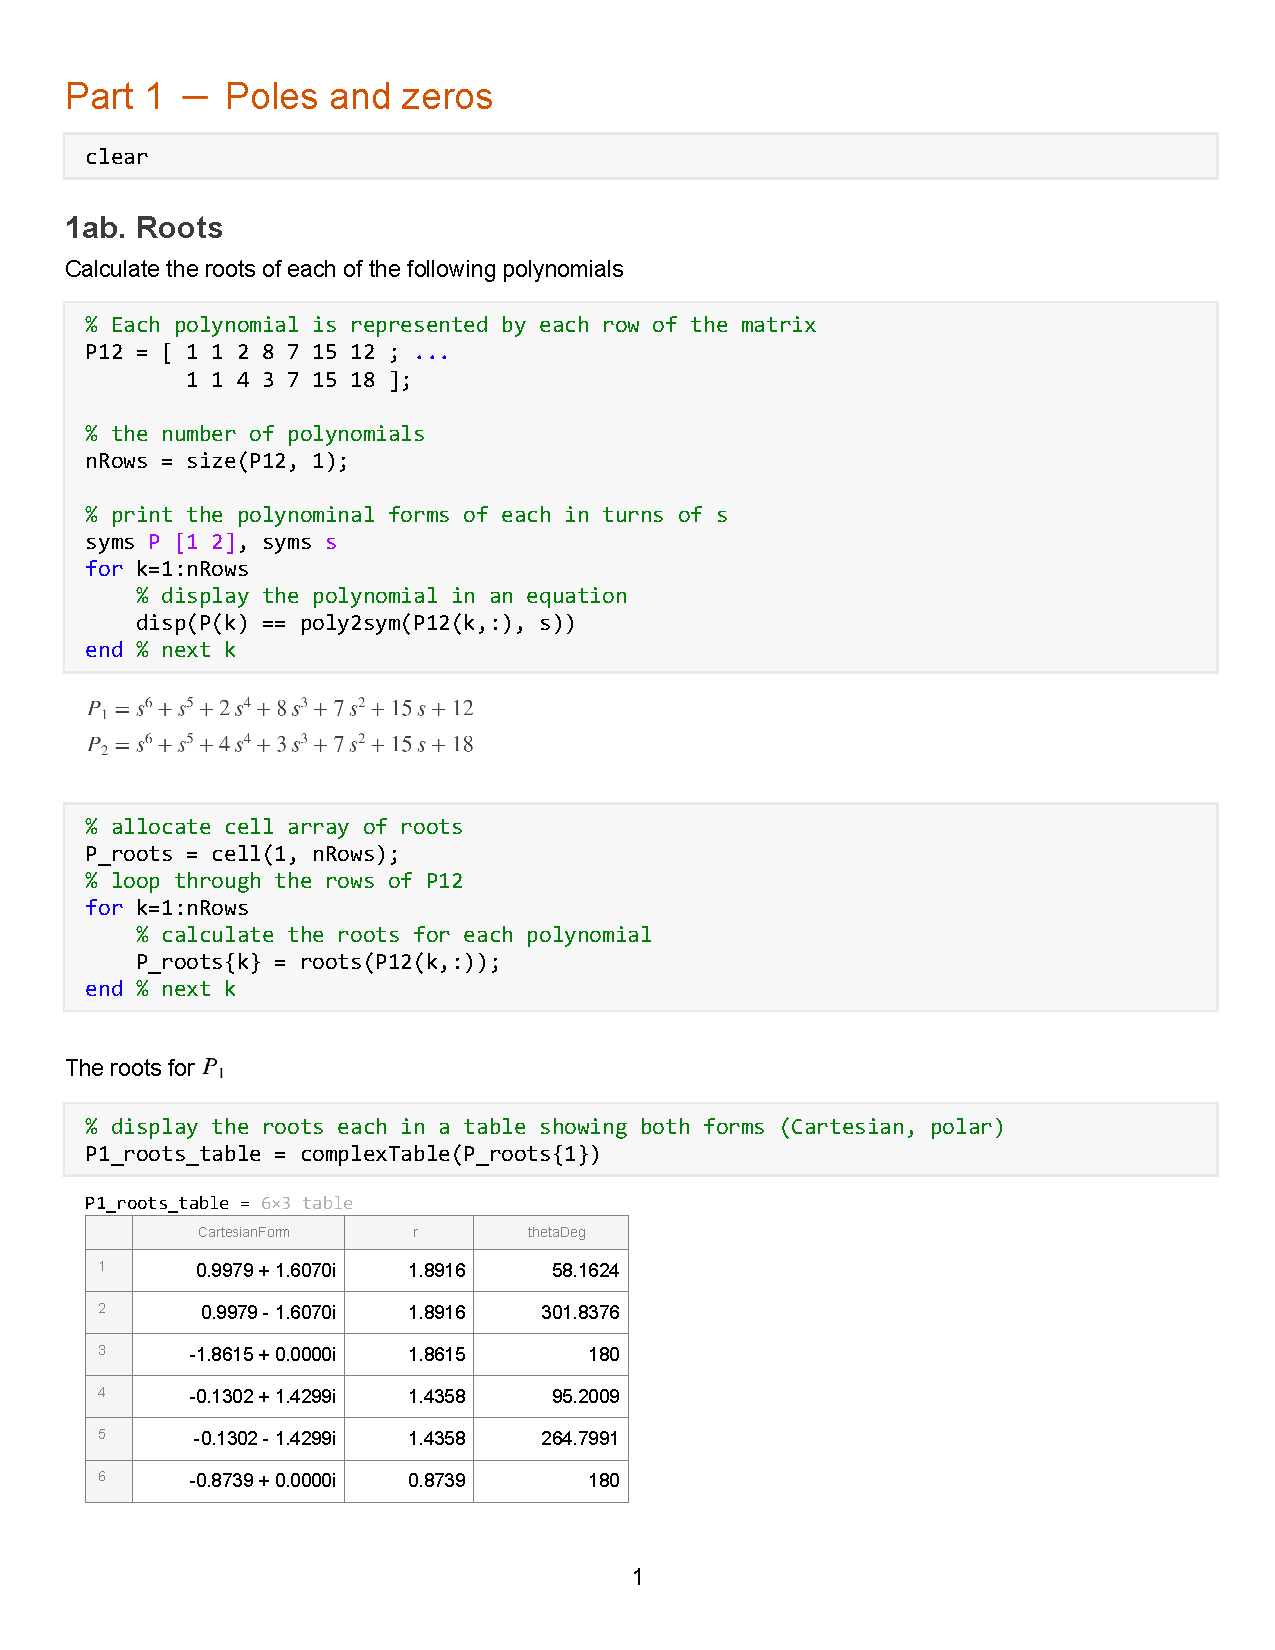
\includepdf[pages={-}]{part01_poles_zeros_mlx.pdf}

\section{Part 2 -- Laplace transforms, Matlab Live Script}

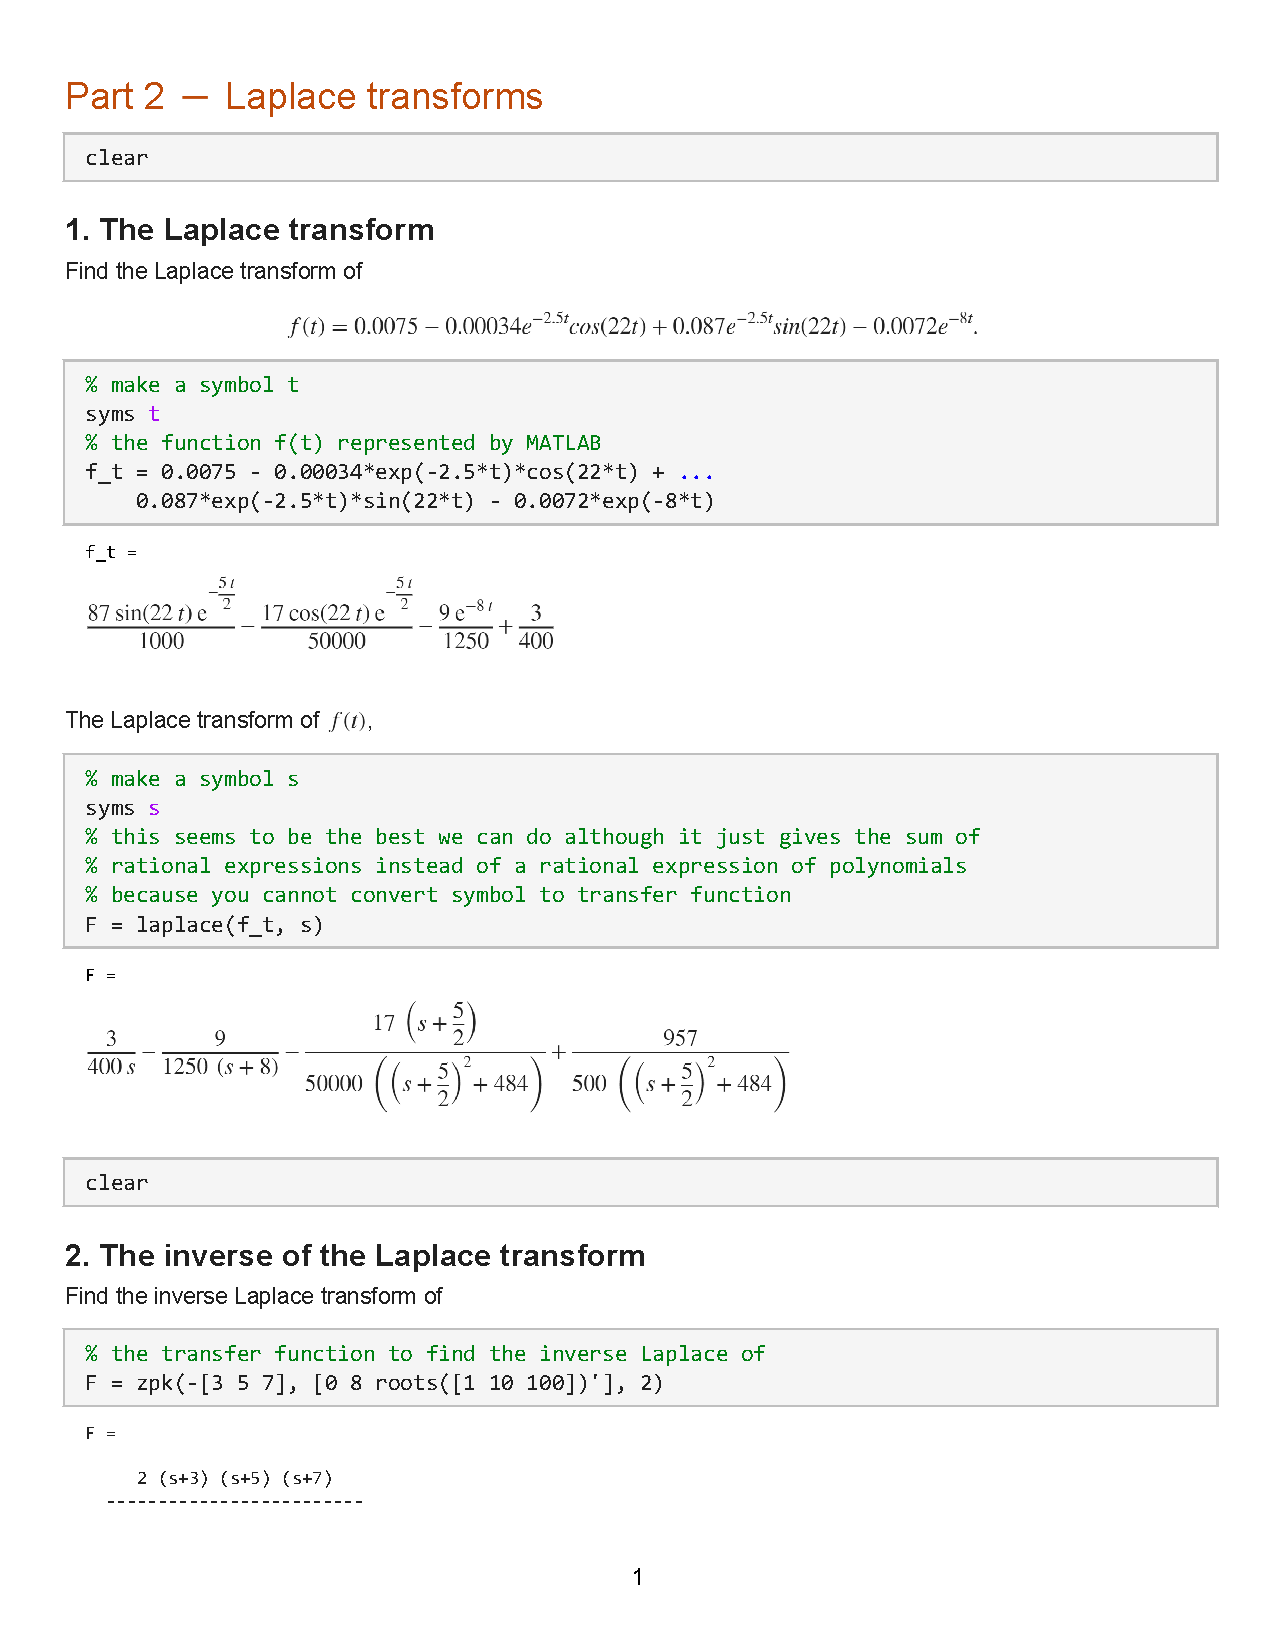
\includepdf[pages={-}]{part02_laplace_transforms_mlx.pdf}

\section{Part 3 -- Review of solving circuit loops, Matlab Live Script}\label{apx:solving circuit loops}

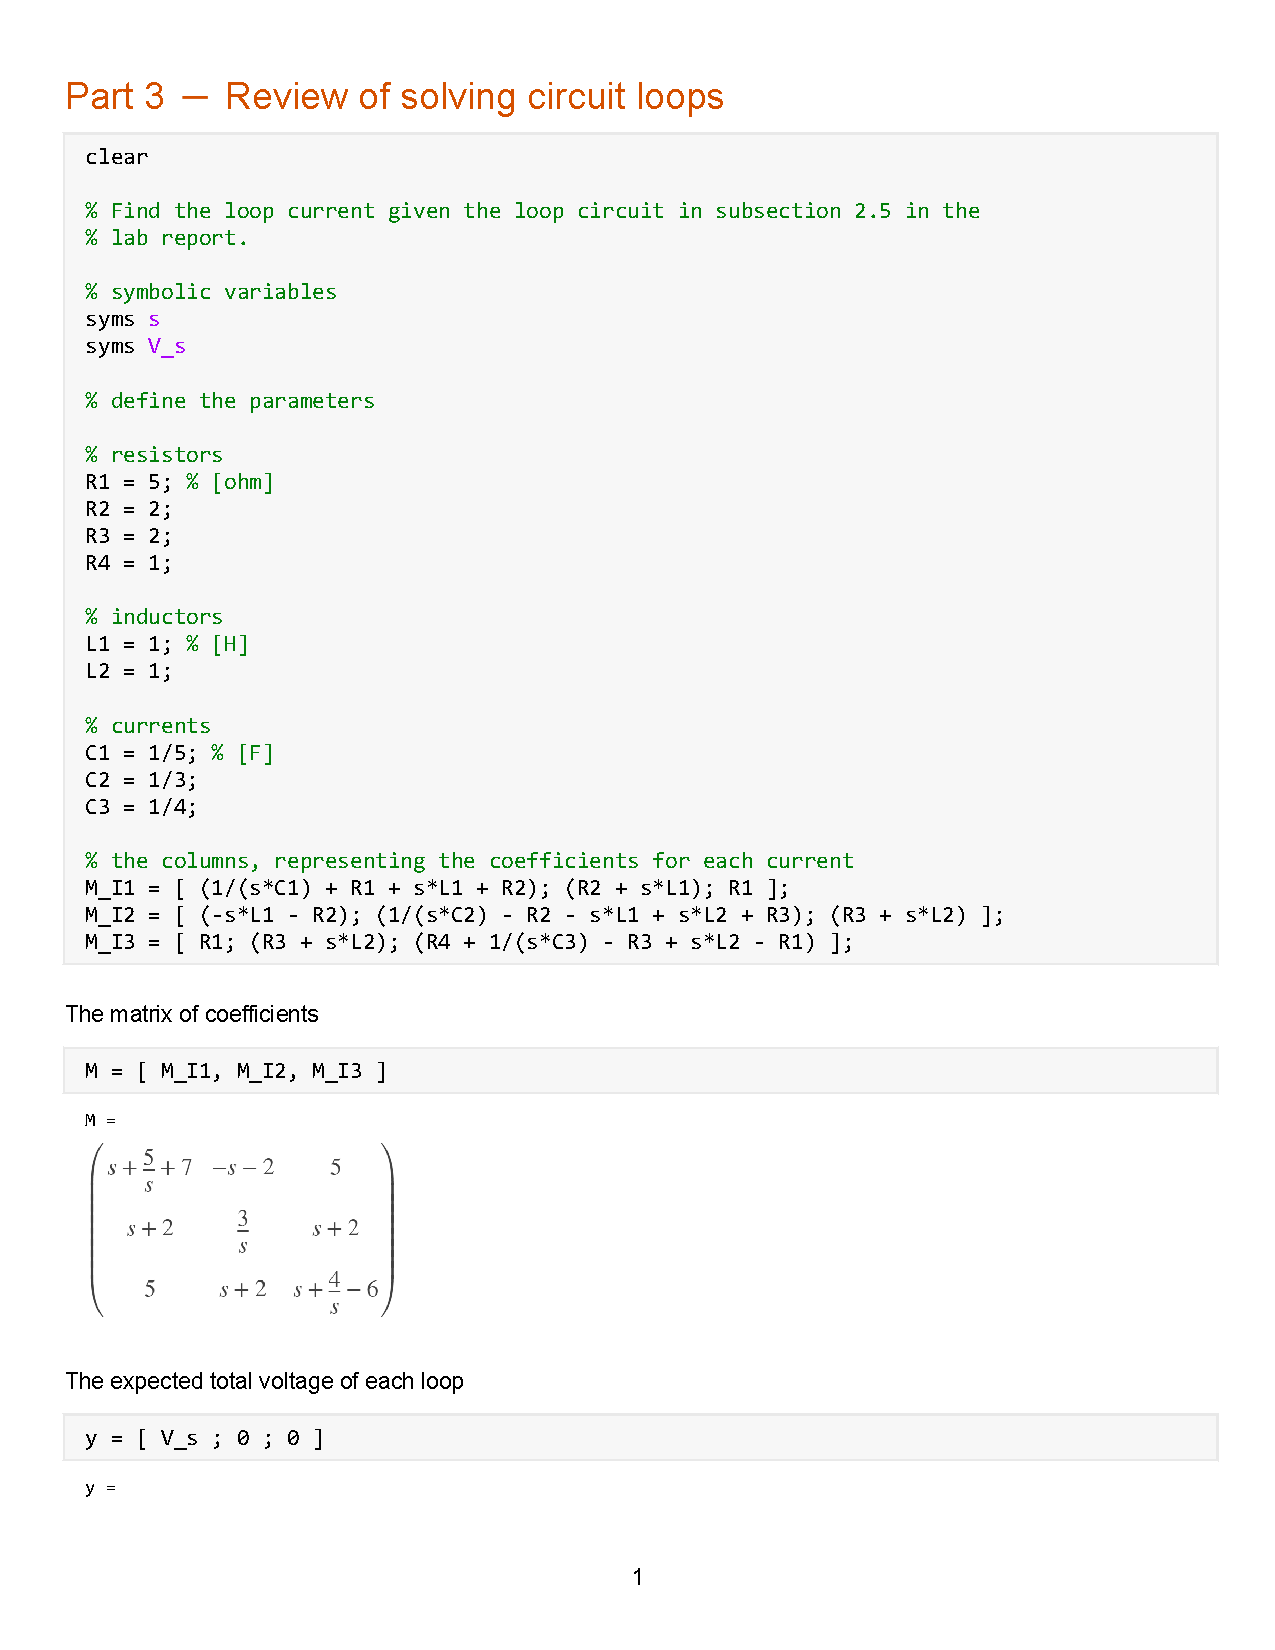
\includepdf[pages={-}]{part03_circuit_loops.pdf}

\end{document}
